\documentclass[a4paper, 12pt]{article}

\usepackage{wrapfig}
\usepackage{graphicx}
\usepackage{mathtext}
\usepackage{amsmath}
\usepackage{siunitx} % Required for alignment
\usepackage{multirow}
\usepackage{rotating}
\usepackage{float}

\usepackage[T1,T2A]{fontenc}
\usepackage[russian]{babel}

\graphicspath{{pictures/}}

\title{\begin{center}Лабораторная работа №1.1.4\end{center}
Измерение интенсивности радиационного фона}
\author{Мыздриков Иван Витаольевич}
\date{3.10.2024}

\begin{document}
    \pagenumbering{gobble}
    \maketitle
    \newpage
    \pagenumbering{arabic}

    \section{Введение}
    \textbf{Цель работы:}
    \begin{itemize}
        \item Применить методы обработки экспериментальных данных для изучения статистических закономерностей при измерении интенсивности радиационного фона
    \end{itemize}

    \vspace{1cm}

    \textbf{В работе используются: }
    \begin{itemize}
        \item счетчик Гейгера-Мюллера
        \item блок питания
        \item компьютер с интерфейсом связи со счетчиком

    \end{itemize}

    \section{Ход работы}
    \paragraph{}
    Проведем измерение используя интерфейс компьютера. Приведем данные в таблицу и начнем  обработку. Разбивая данные для 20с по парам и просуммировав пары получим данные для 40с.
    \paragraph{}
    Проверим связь $\sigma_{отд}\approx \sqrt{\bar{n}}$. Индекс 1 для 10с, 2 для 40с
    \[n_{общ} = \sum n_i = 5403\]
    \[\bar{n}_1 = \frac{n_{общ}}{N_1} = 13.50\]
    \[\bar{n}_2 = \frac{n_{общ}}{N_2} = 54.03\]
    \[\sigma_{1}=\sqrt{\frac{1}{N_1} \sum_{i=1}^{N_1} (n_i - \bar{n}_i)^2} \approx 3.67\]
    \[\sigma_{2}=\sqrt{\frac{1}{N_2} \sum_{i=1}^{N_2} (n_i - \bar{n}_i)^2} \approx 6.83\]
    \newpage

    \[\sqrt{\bar{n}_1} =3.67 \approx 3.67= \sigma_1\]
    \[\sqrt{\bar{n}_2} =7.34 \approx 6.83 = \sigma_2\]
    \paragraph{}
    Как видим связь между среднеквадратическим отклонением и среднем значении есть $(\sigma \approx \sqrt{\bar{n}})$.
    Теперь определим долю случаев в пределах $\pm\sigma$ и $\pm2\sigma$.

    \begin{table}[H]
    \begin{center}
    \begin{tabular}{|c|c|c|c|}\hline
    \multicolumn{4}{|c|}{$t=10с$}\\\hline
    Предел & Число случаев & Доля случаев & Теоретическая оценка\\\hline
    $\pm \sigma_1 = \pm 3.7$ & 291 & 70\% & 68\% \\
    $\pm 2\sigma_1 = \pm 7.6$ & 385 & 96\% & 95\% \\\hline
    \multicolumn{4}{c}{}\\\hline
    \multicolumn{4}{|c|}{$t=10с$}\\\hline
    Предел & Число случаев & Доля случаев & Теоретическая оценка\\\hline
    $\pm \sigma_2 = \pm 6.8$ & 66 & 66\% & 68\% \\
    $\pm 2\sigma_2 = \pm 13.6$ & 97 & 97\% & 95\% \\\hline

    \end{tabular}
    \caption{Количество измерении за пределами $\pm\sigma$ и $\pm2\sigma$}
    \end{center}
    \end{table}

    \paragraph{}
    Как видим наши данные с довольно хорошей точностью соответствуют теории. Как видно из графика относительный разброс данных за 40с меньше чем за 10с. Подсчитаем какая разница между этими 2мя случаями.
    \[\frac{\sigma_1}{\bar{n}_1} \approx 28\%, \frac{\sigma_2}{\bar{n}_2} \approx 12\%\]
    \paragraph{}
    Как видим разница почти в 2 раза, что и следует от того факта что $\sigma \approx \sqrt{\bar{n}}$.
    \paragraph{}
    Для финалбного ответа подсчитаем ошибки средних величин. По теории
    \[\sigma_{\bar{n}_1} = \frac{\sigma_{1}}{\sqrt{N_1}} \approx 0.18, \sigma_{\bar{n}_2} \approx 0.68\]
    \[\varepsilon_{\bar{n}_1} = \frac{\sigma_{\bar{n}_1}}{\bar{n}_1}\approx 1.3\%, \varepsilon_{\bar{n}_2}\approx 1.3\%\]
    Получаем финальный результат
    \[n_{t=10с}=13.5 \pm 0.18\]
    \[n_{t=40с}=54.05 \pm 0.68\]

    \newpage
    \begin{table}[H]
    \begin{center}
    \begin{tabular}{|c|r|r|r|r|r|r|r|r|r|r|}
    \hline
    {№ опыта} &   1 &   2 &   3 &   4 &   5 &   6 &   7 &   8 &   9 &  10 \\
    \hline
    0 & 28 & 24 & 26 & 30 & 31 & 27 & 29 & 23 & 22 & 29 \\
    1 & 23 & 31 & 36 & 28 & 22 & 21 & 20 & 18 & 17 & 28 \\
    2 & 27 & 45 & 31 & 22 & 18 & 27 & 26 & 30 & 31 & 28 \\
    3 & 24 & 20 & 21 & 26 & 24 & 26 & 27 & 29 & 27 & 19 \\
    4 & 28 & 22 & 38 & 25 & 30 & 25 & 26 & 26 & 35 & 37 \\
    5 & 31 & 32 & 22 & 24 & 23 & 32 & 27 & 33 & 25 & 25 \\
    6 & 25 & 22 & 26 & 28 & 34 & 18 & 30 & 24 & 33 & 24 \\
    7 & 30 & 28 & 24 & 26 & 29 & 25 & 31 & 27 & 33 & 21 \\
    8 & 31 & 26 & 24 & 23 & 34 & 26 & 30 & 33 & 17 & 31 \\
    9 & 23 & 21 & 25 & 29 & 31 & 28 & 26 & 21 & 27 & 35 \\
    10 & 23 & 30 & 30 & 20 & 40 & 15 & 19 & 34 & 24 & 22 \\
    11 & 38 & 29 & 35 & 26 & 27 & 24 & 40 & 27 & 27 & 39 \\
    12 & 30 & 25 & 23 & 33 & 27 & 21 & 24 & 30 & 35 & 33 \\
    13 & 25 & 28 & 22 & 26 & 32 & 23 & 34 & 32 & 22 & 27 \\
    14 & 35 & 31 & 36 & 33 & 29 & 22 & 30 & 31 & 19 & 19 \\
    15 & 26 & 25 & 20 & 26 & 30 & 19 & 26 & 23 & 31 & 25 \\
    16 & 21 & 30 & 23 & 25 & 28 & 17 & 29 & 26 & 26 & 36 \\
    17 & 20 & 28 & 36 & 24 & 36 & 21 & 23 & 23 & 26 & 19 \\
    18 & 21 & 27 & 26 & 26 & 30 & 37 & 33 & 26 & 25 & 25 \\
    19 & 30 & 25 & 23 & 22 & 26 & 30 & 26 & 35 & 23 & 27 \\
    \hline
    \end{tabular}
    \caption{Число срабатывании счетчика за 20с}
    \end{center}
    \end{table}


    \begin{table}[H]
    \begin{center}
    \begin{tabular}{|l|c|c|c|c|c|c|c|}\hline
    Число импульсов & 5 & 6 & 7 & 8 & 9 & 10 & 11  \\\hline
    Число случаев & 3 & 3 & 9 & 16 & 26 & 27 & 45 \\\hline
    Доля случаев & 0.0075 & 0.0075 & 0.0225 & 0.04 & 0.065 & 0.0675 & 0.1125 \\\hline
    \multicolumn{8}{c}{}\\\hline
    Число импульсов & 12 & 13 & 14 & 15 & 16 & 17 & 18 \\\hline
    Число случаев & 41 & 35 & 36 & 41 & 37 & 29 & 15 \\\hline
    Доля случаев & 0.1025 & 0.0875 & 0.09 & 0.1025 & 0.0925 & 0.0725 & 0.0375 \\\hline
    \multicolumn{8}{c}{}\\\hline
    Число импульсов & 19 & 20 & 21 & 22 & 23 & 24 & 26  \\\hline
    Число случаев & 10 & 14 & 6 & 3 & 1 & 2 & 1  \\\hline
    Доля случаев & 0.025 & 0.035 & 0.015 & 0.0075 & 0.0025 & 0.005 & 0.0025  \\\hline
    \end{tabular}
    \caption{Данные для построения гистограммы для 10с}
    \end{center}
    \end{table}
    \newpage

    \begin{table}[H]
    \begin{center}
    \begin{tabular}{|c|r|r|r|r|r|r|r|r|r|r|}
    \hline
    {№ опыта} &   1 &   2 &   3 &   4 &   5 &   6 &   7 &   8 &   9 &  10 \\
    \hline
    0 & 51 & 51 & 59 & 55 & 54 & 61 & 55 & 61 & 41 & 51 \\
    10 & 55 & 65 & 54 & 50 & 47 & 59 & 53 & 56 & 58 & 52 \\
    20 & 62 & 52 & 60 & 50 & 49 & 65 & 45 & 56 & 59 & 49 \\
    30 & 58 & 48 & 49 & 54 & 52 & 46 & 59 & 59 & 49 & 48 \\
    40 & 53 & 42 & 53 & 63 & 65 & 67 & 59 & 59 & 64 & 56 \\
    50 & 48 & 53 & 57 & 43 & 54 & 39 & 44 & 41 & 38 & 67 \\
    60 & 49 & 53 & 53 & 61 & 56 & 59 & 58 & 56 & 52 & 59 \\
    70 & 41 & 59 & 59 & 51 & 54 & 61 & 62 & 54 & 49 & 61 \\
    80 & 39 & 58 & 60 & 66 & 44 & 51 & 57 & 50 & 52 & 48 \\
    90 & 57 & 47 & 62 & 45 & 66 & 61 & 60 & 44 & 55 & 52 \\
    \hline
    \end{tabular}
    \caption{Число срабатывании счетчика за 40с}
    \end{center}
    \end{table}

    \begin{table}[H]
    \begin{center}
    \begin{tabular}{|l|c|c|c|c|c|c|c|c|c|c|}\hline
    Число импульсов & 38.0 & 39.0 & 41.0 & 42.0 & 43.0 & 44.0 & 45.0 & 46.0 & 47.0 & 48.0 \\\hline
    Число случаев & 1.0 & 2.0 & 3.0 & 1.0 & 1.0 & 3.0 & 2.0 & 1.0 & 2.0 & 4.0 \\\hline
    Доля случаев & 0.01 & 0.02 & 0.03 & 0.01 & 0.01 & 0.03 & 0.02 & 0.01 & 0.02 & 0.04 \\\hline
    \multicolumn{11}{c}{}\\\hline
    Число импульсов & 49.0 & 50.0 & 51.0 & 52.0 & 53.0 & 54.0 & 55.0 & 56.0 & 57.0 & 58\\\hline
    Число случаев & 6.0 & 3.0 & 5.0 & 6.0 & 6.0 & 6.0 & 4.0 & 5.0 & 3.0 & 4.0 \\\hline
    Доля случаев & 0.06 & 0.03 & 0.05 & 0.06 & 0.06 & 0.06 & 0.04 & 0.05 & 0.03 & 0.04 \\\hline
    \multicolumn{10}{c}{}\\\hline
    Число импульсов & 59.0 & 60.0 & 61.0 & 62.0 & 63.0 & 64.0 & 65.0 & 66.0 & 67.0  \\\hline
    Число случаев & 11.0 & 3.0 & 6.0 & 3.0 & 1.0 & 1.0 & 3.0 & 2.0 & 2.0  \\\hline
    Доля случаев & 0.11 & 0.03 & 0.06 & 0.03 & 0.01 & 0.01 & 0.03 & 0.02 & 0.02  \\\hline
    \end{tabular}
    \caption{Данные для построения гистограммы для 40с}
    \end{center}
    \end{table}
    \newpage

    \begin{sidewaysfigure}
        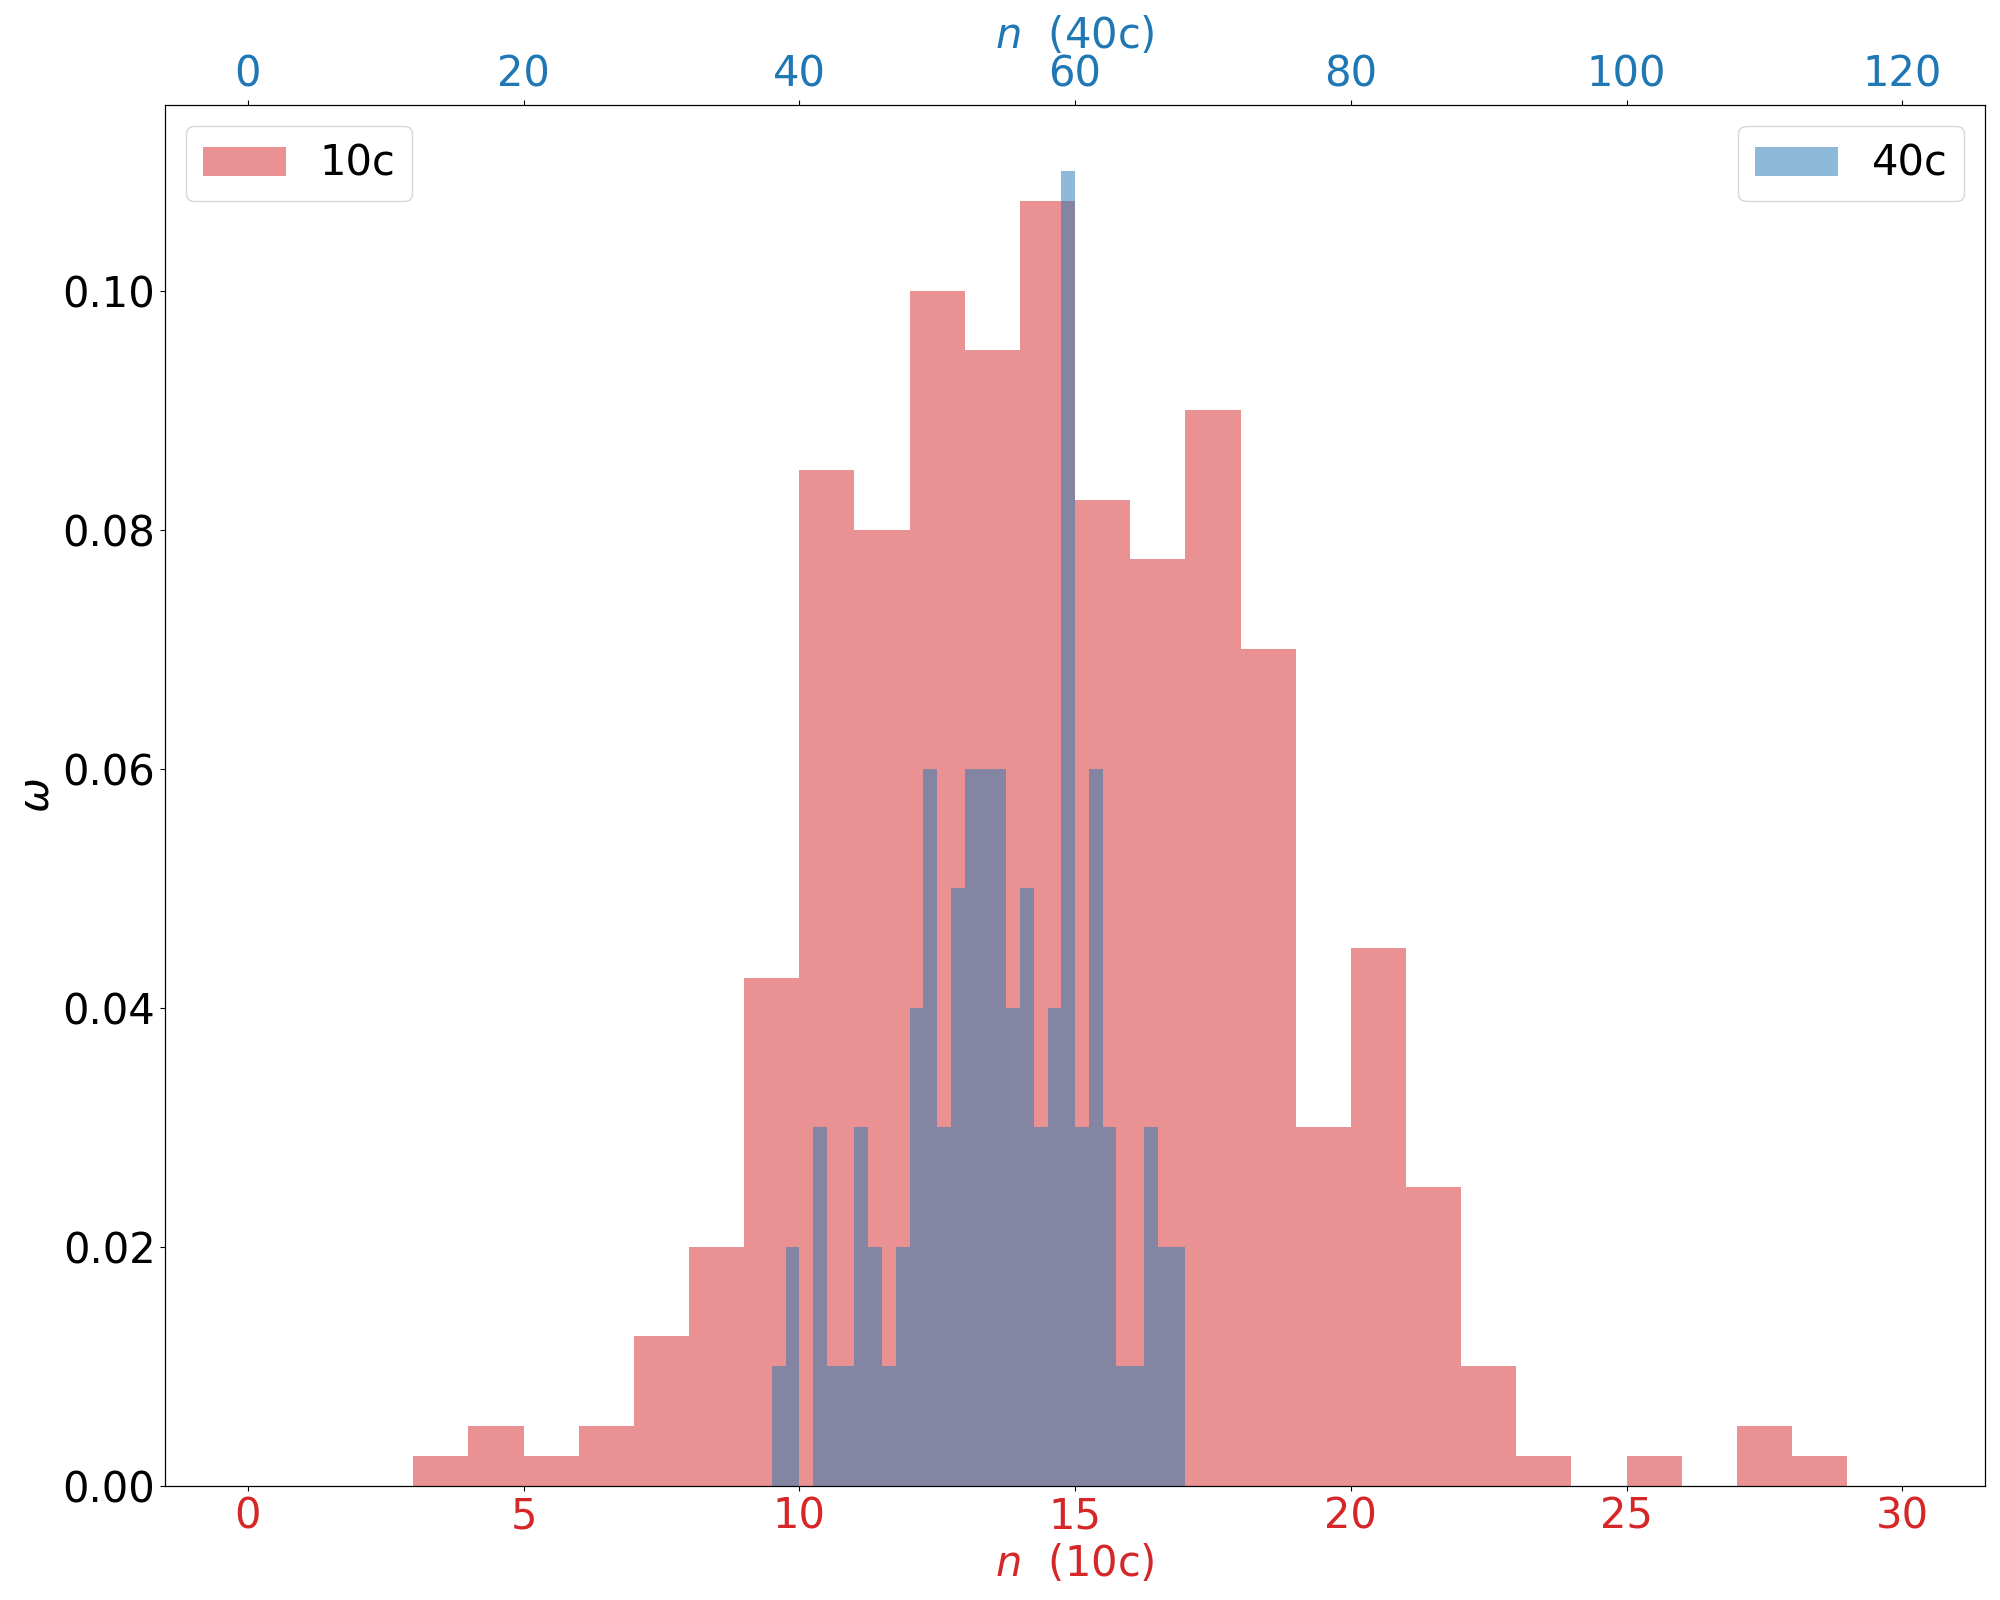
\includegraphics[scale=0.45]{histogram.png}
        \caption{Гистограммы для $t=10с$ и $t=40с$}
    \end{sidewaysfigure}
\end{document}
